\chapter{Background}

This chapter explores the evolution of Android and introduces its architecture. Although Android is built on top of Linux kernel, it has become an operating system in a class by itself. Android introduces a vast collection of frameworks, as well as a runtime (Dalvik/ART) to support them. We then turn to examine the Android architecture, each layer is described in detail to set the foundation for the deeper exploration carried out in the next chapters of this work. Finally, we consider and discuss in detail 

\section{Android}

%Android is an open source operating system with open architecture where apps are published at numerous third-party market along with its official app market, i.e., Google Play store. Google Play store surpassed 2.6 million apps in December 2016. 

Android is a modern operating system with a layered software stack. The following Figure \ref{fig:androidsys} illustrates the layers in Android's software stack. This software stack runs on top of the device hardware. Android's software stack can run on many different hardware configurations

\begin{figure}[H]
\centering
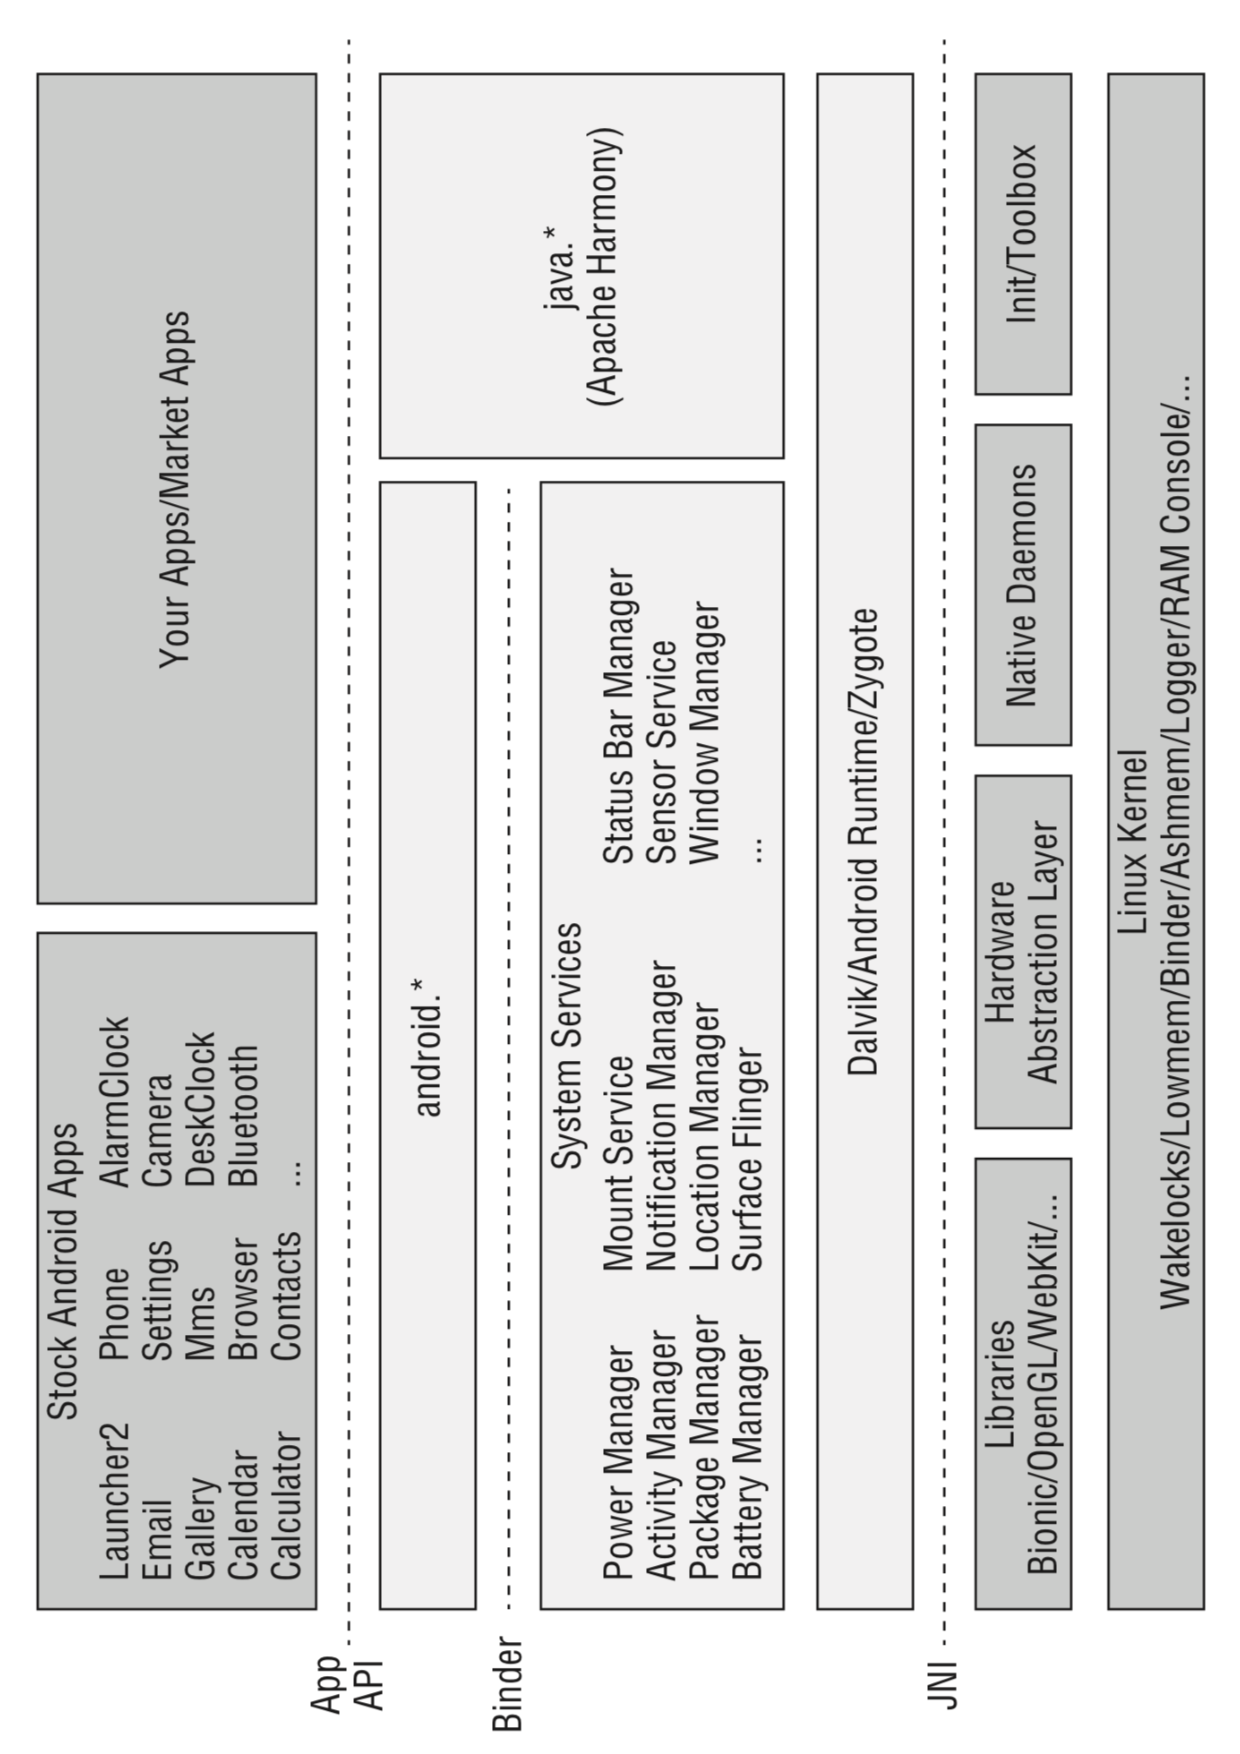
\includegraphics[width=.5\textwidth, keepaspectratio, resolution=600]{android-stack.pdf}
\caption{Android System Architecture}
\label{fig:androidsys}
\end{figure}

Most of the user-facing features and enhancements in between versions have to do with additional frameworks and APIs being added, with only a relatively small portion of them at the system level. At the time of writing the latest Android version is Oreo 8.1, API number 27. 

Android applications allow developers to extend and improve the functionality of a device without having to alter lower levels. In turn, the Android Framework provides developers with a rich API that has access to all of the various facilities an Android device has to offer. This includes building blocks to enable developers to perform common tasks such as managing user interface (UI) elements, accessing shared data stores, and passing messages between application components.

The Android OS is based on a Linux kernel but offers a different application abstraction than found in traditional Linux distributions. Android apps are mostly written in Java and compiled into Dalvik bytecode to be executed by the Dalvik Virtual Machine (DVM). Apps may optionally contain native code components. Newer versions of Android \footnote{\url{https://source.android.com/devices/tech/dalvik/}} employ the Android Run Time (ART) that converts bytecode to native code at install time (Ahead Of Time compilation). Android apps are distributed as an APK file that basically is a ZIP file containing the app's bytecode (in \textit{classes.dex}) and its resources. 

The Android operating system utilizes two separate, but cooperating, permissions models. At the low level, the Linux kernel enforces permissions using users and groups. This permissions model is inherited from Linux and enforces access to  le system entries, as well as other Android specific resources. This is commonly referred to as Android’s sandbox (see XXX).

Although each app executes within a dedicated process space, Android allows apps to communicate with each other through a well-defined Inter-Process Communication (IPC) mechanism, referred to as Binder. It provides message passing (called \textit{parcels}) taking care of migrating the execution of a request from the requester to the target process transparently to the apps. The Binder system includes a kernel module, accessed through the \texttt{/dev/binder} file. Communications between different components in the same app are handled by the Binder. 

\subsection*{Android Framework}

The glue between apps and the runtime, the Android Framework provides the pieces —packages and their classes- for developers to perform common tasks. Such tasks might include managing UI elements, accessing shared data stores, and passing messages between application components. 

The common framework packages are those within the android.* namespace, such as android.content or android.telephony. Android also provides many standard Java classes (in the java.* and javax.* namespaces), as well as additional third-party packages. The Android Framework also includes the services used to manage and facilitate much of the functionality provided by the classes within. The framework includes the basic blocks for building Android applications.

Even though almost all Android OS functionality above the kernel level is implemented as system services, it is not exposed directly in the framework but is accessed via facade classes called managers. Typically, each manager is backed by a corresponding system service; for example, the BluetoothManager is a facade for the BluetoothManagerService.  System services (79 as of version 4.4) implement most of the fundamental Android features, including display and touch screen support, telephony, and network connectivity. fundamental ones are written in native code.

With a few exceptions, each system service defines a remote interface that can be called from other services and applications. Coupled with the service discovery, mediation, and IPC provided by Binder, system services effectively implement an object-oriented OS on top of Linux.

\subsection*{Android Binder}

While Android’s Binder is a new implementation, it’s based on the architecture and ideas of OpenBinder.
The Binder driver is the central object of the framework, and all IPC calls
go through it. Inter-process communication is implemented with a single ioctl() call that both sends and receives data through the $binder\_write\_read$ structure.
%which consists of a write_buffer containing commands for the driver, and a read_buffer containing commands that the userspace needs to perform.

Binder acts as a mediation point for all IPC. Access to system resources (e.g., GPS receivers, text messaging, phone services, and the Internet), data (e.g., address books, email) and IPC is governed by permissions as- signed at install time. The permissions requested by the application and the permissions required to access the application’s interfaces/data are defined in its manifest file.

\begin{figure}[H]
\centering
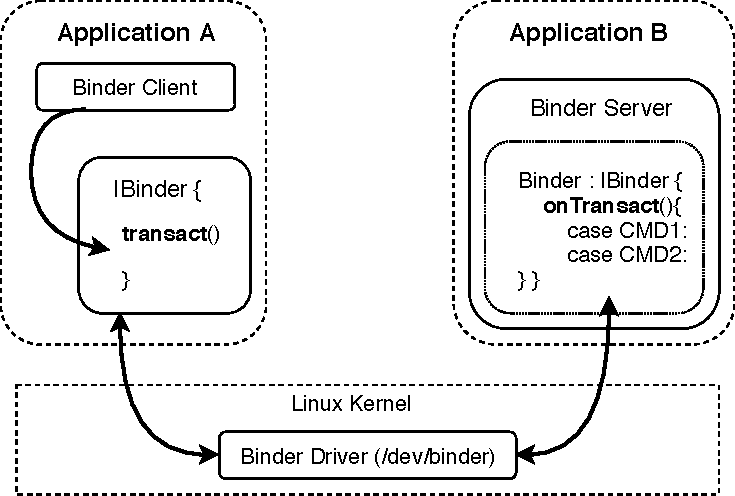
\includegraphics[width=.5\textwidth, keepaspectratio, resolution=600]{bindersys.pdf}
\caption{Android Binder Mechanism}
\label{fig:androidmodel}
\end{figure}

When a process sends a message to another process, the kernel allocates some space in the destination process’s memory, and copies the message data directly from the sending process. It then queues a short message to the receiving process telling it where the received message is. The recipient can then access that message directly (because it is in its own memory space). When a process is  finished with the message, it notifies the Binder driver to mark the memory as free.

Higher-level IPC abstractions in Android such as Intents (commands with associated data that are delivered to components across processes), Messengers (objects that enable message-based communication across processes), and ContentProviders (components that expose a cross-process data management interface) are built on top of Binder. Additionally, service interfaces that need to be exposed to other processes can be de ned using the Android Interface De nition Language (AIDL), which enables clients to call remote services as if they were local Java objects. The associated aidl tool automatically generates stubs (client-side representations of the remote object) and proxies that map interface methods to the lower-level transact() Binder method and take care of converting parameters to a format that Binder can transmit (this is called parameter marshalling/unmarshalling). Because Binder is inherently typeless, AIDL-generated stubs and proxies also provide type safety by including the target interface name in each Binder transaction (in the proxy) and validating it in the stub.

\subsection*{Android Application} 

While all apps have the same structure and are built on top of the Android framework, we distinguish between system apps and user-installed apps. System apps are included in the OS image, which is read-only on production devices (typically mounted as /system), and cannot be uninstalled or changed by users. Therefore, these apps are considered secure and are given many more privileges than user-installed apps. System apps can be part of the core Android OS or can simply be pre-installed user applications, such as email clients or browsers. User-installed apps are installed on a dedicated read-write partition (typically mounted as /data) that hosts user data and can be uninstalled at will. Each application lives in a dedicated security sandbox and typically cannot affect other applications or access their data. Additionally, apps can only access resources that they have explicitly been granted a permission to use. Privilege separation and the principle of least privilege are central to Android’s security model, and we will explore how they are implemented in the next section. 


Android apps are organised in components\footnote{\url{https://developer.android.com/guide/components/index.html}} that permit to achieve different functionalities. Android offers four types of components: Activity,  Content Provider, Service and Broadcast Receiver. The app's user interface is composed of a sets of activity components. Content provider components offer per-application data servers that are queried by other installed apps. Service components are intended for background processing. Broadcast receiver components handle asynchronous messages across apps as well as Android system. An Android Intent\footnote{\url{https://developer.android.com/guide/components/intents-filters.html}} is used as a messaging object to request an action from another app component. Although intents facilitate communication between components in several ways, there are three fundamental use cases: starting an activity, a service or delivering a broadcast message. 


Android apps require to define a special file called \texttt{AndroidManifest.xml}, known as manifest\cite{manifest}, that contains specific meaningful information about the related Android app. Every app must have a manifest file in its root directory because the Android system needs to access its content before it can run any of the app's code. As a consequence, the manifest file cannot be obfuscated. The information declared in the manifest  cannot be changed at runtime: even  dynamically loaded code must comply with the permissions and the components defined in the app's manifest.

\textbf{Android \texttt{sharedUserId} attribute.} The manifest attribute \shared, introduced since the first Android version, is a feature that allows to execute different apps under the same UID if and only if they are signed with the same certificate. Once installed, apps that share the same UID will have access to each other private data because they share the same Linux permissions set. This feature is extensively used by Android for core framework services and system apps. For instance, the Play Service and the Google location service use the \shared to request to run in the same process of the login service to be able to sync data in the background, without  user interaction. This feature is available to and widely used also by third-party developers to update their apps and shared libraries. Removing such features will have  an important impact on backward compatibility.
  
\textbf{Android \texttt{process} attribute.} The attribute \proc allows to execute two different apps within the same process space. It can be specified for any components in an app. Whenever the execution of  a component is requested, Android first looks for a running process matching the name specified in \proc. If a process is found, then that process will be used to execute the requested component. This avoids spawning a new process for a component if there is already a running instance of that component. For instance, this is used to reuse the background activity's process when it is called in foreground again.

\textbf{Java Native Interface.} Android Application allows the inclusion of native libraries (ELF shared objects) in application code, through the Java Native Interface (JNI).
From the Linux perspective, all executables are ELF binaries. It is therefore not at all uncommon to see JNI used in applications optimizing for performance, or seeking resistance to reverse engineering. Google therefore provides the Native Development Kit (NDK) (                Android Developer), which developers can use to build native libraries (and binaries). Android's critical system  component are implemented in C/C++, and are compiled into native binaries. User applications are compiled into Dalvik bytecode, but the bytecode runs (or, in ART, is compiled ahead-of- time) in the context of a Dalvik Virtual machine, which is, in and of itself, an ELF binary. Thus, while most developers remain oblivious to binaries, they nonetheless play an important role in Android.



\subsection*{Android Security Model} 
Android provides a sandbox for each installed app, as shown in Figure \ref{fig:androidmodel}. To enforce this isolation at the Linux kernel, Android assigns at install time a unique User ID (UID) to each app. 

Moreover, since Android version 4.3, SELinux was adopted with its Mandatory Access Control (MAC) model in order  to enforce a more fine-grained UID-based isolation and to harden the OS components mitigating the risk of flawed and malicious code.  In addition, Android combines the traditional Linux permissions with a Mandatory Access Control (MAC) mechanism at framework level. During install time, apps are assigned permission labels representing the resources they can access during runtime. The developer of an app must declare the permissions the app requires in its manifest file. SELinux can operate in one of two global modes: permissive mode, in which permission denials are logged but not enforced, and enforcing mode, in which denials are both logged and enforced. SELinux also supports a per-domain permissive mode in which specific domains (processes) can be made permissive while placing the rest of the system in global enforc- ing mode. In the Android 5.0 L release, Android moves to full enforcement of SELinux. This builds upon the permissive release of 4.3 and the partial enforcement of 4.4. In short, Android is shifting from enforcement on a limited set of crucial domains (installd, netd, vold and zygote) to everything.

\begin{figure}[H]
\centering
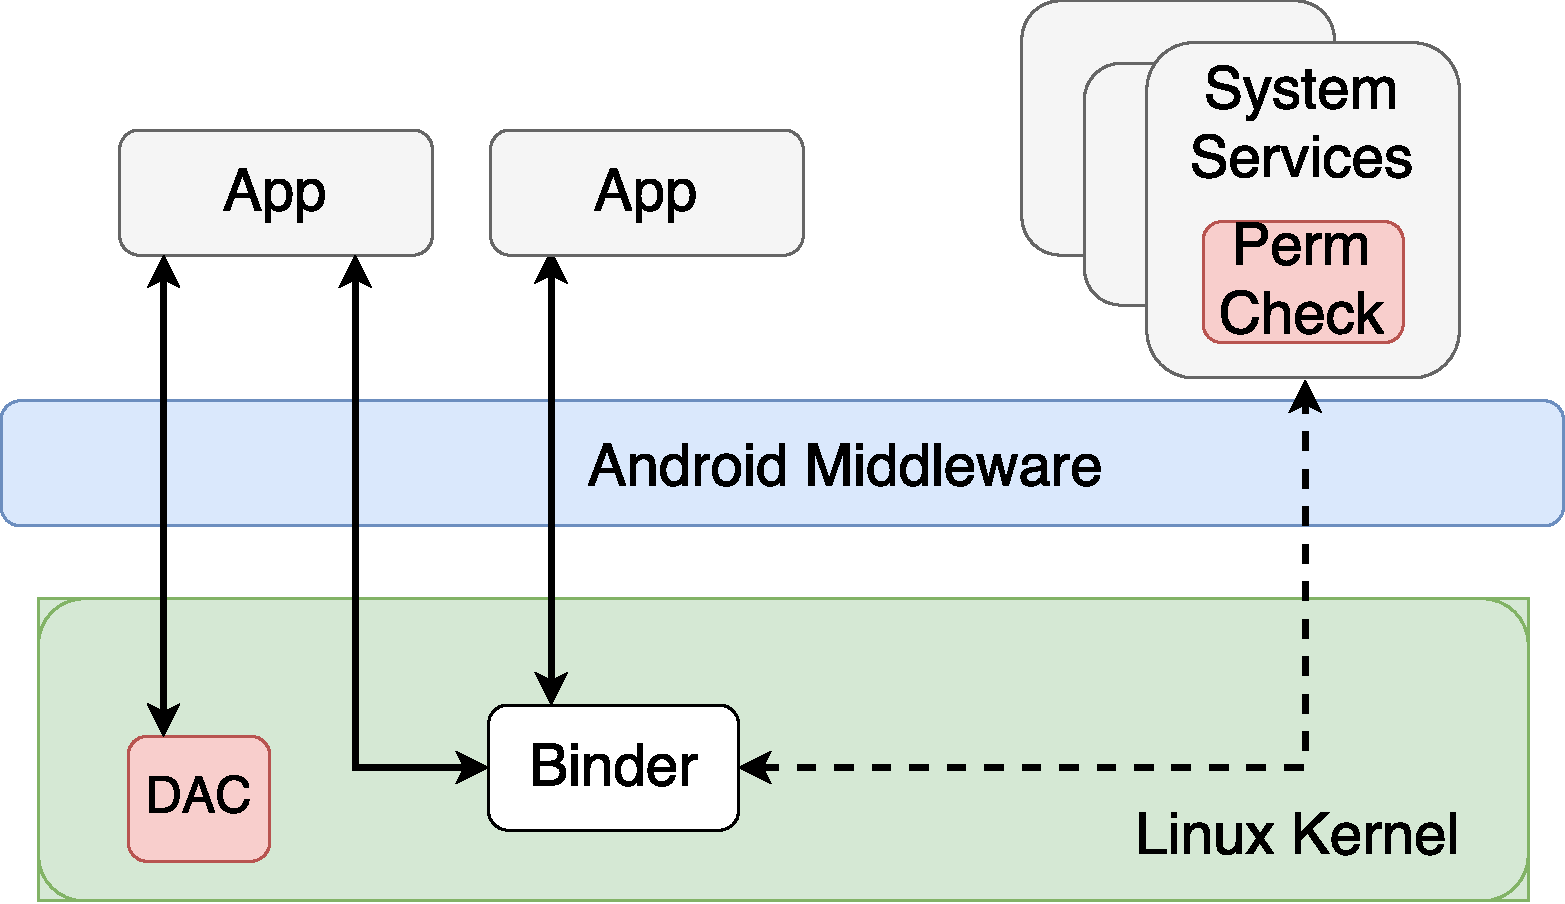
\includegraphics[width=.5\textwidth, keepaspectratio, resolution=600]{android_model}
\caption{Android Security model}
\label{fig:androidmodel}
\end{figure}

%\textbf{Apps certificate.}  
Android requires  all APKs to be digitally signed with a certificate. A public-key certificate contains the public key of a public/private key pair, as well as some other metadata identifying the owner of the key. The owner of the certificate holds the corresponding private key. When a developer signs an APK, the signing tool attaches the public-key certificate to the produced APK. The public-key certificate serves as a fingerprint that uniquely associates the APK to its developer and his corresponding private key. This helps Android to ensure that any future updates to that APK  come from the original developer. In fact, developers must use the same certificate throughout the lifespan of their apps to push new versions of their apps to the users' devices. In Android, a certificate authority is not mandatory: typically the app certificates do not need to be signed by a certificate authority and most developers use self-signed certificates.

%During a 30-day active user monitoring in September 2015, Google confirmed that Android has 1.4 billion active users globally. Android operative system has been expanding across different market segments which include automotive, smart tv and wearable devices. Dominating the smartphone market for the last few years, it reached 86.2\% of the smartphone market share in 2016. Mobile computing has gone from a niche market of gadget-driven consumers to the fastest growing way for users to perform office work, undertake banking transactions, remain active on their social networks, and much more, on the move. 


%The Android OS makes use of a peculiar Inter Process Communication (IPC) mechanism which has its core in the Binder component. The Binder takes care of inter-application communications as well as of intra-application ones, in fact spawning an app's internal activity  involves IPC messages with the \textit{ActivityManager} component. This mechanism plays a core role in the whole Android platform, allowing messages passing forward and backward from privileged services and user applications it allows to define system services in charge of enforcing the permissions offered by Android platform and granted by the user to that specific application. As any modern mobile operative system also Android is highly tied to user interaction offering ways to manage running apps, putting them in foreground execution, handling user input in many different means (i.e., gyroscopic, accelerometer, video camera, microphone). Moreover, Android is highly even-based which means that for instance receiving and sms or a call produces a specific event that will be sent in broadcast to all registered applications.